\documentclass[12pt,a4paper,oneside, titlepage]{article}
\usepackage[left=2cm,right=2cm,top=2cm,bottom=2cm]{geometry}
\usepackage[pdftex]{graphicx}
\usepackage[final]{pdfpages}
%\usepackage[frenchb]{babel}
\usepackage[utf8]{inputenc}
\usepackage{cite}
\usepackage{hyperref}
\usepackage{amsmath}
\usepackage{amsthm}
\begin{document}
\newcommand{\spherotitle}[2]{
\begin{titlepage}
\begin{center}

\includegraphics[scale=1.50]{../UMONS.jpg}\\[0.4cm]

\includegraphics[scale=0.30]{../FS_Logo.jpg}\\[3cm]
{\Large Un réseau de neurones pour la}\\

\includegraphics[scale=0.30]{../sphero.jpg}\\
\rule{8cm}{0.5mm}\\[0.5cm]
{\huge \bfseries #1}\\[0.2cm]
\rule{8cm}{0.5mm}\\[7cm]
% Author and supervisor. Come from http://www.jujens.eu/posts/2013/Oct/20/latex-page-garde/
    \begin{minipage}{0.4\textwidth}
      \begin{flushleft} \large
        Jason \textsc{Bury}\\
        130538\\
        Master 1 en\\Science-informatique\\
      \end{flushleft}
    \end{minipage}
    \begin{minipage}{0.4\textwidth}
      \begin{flushright} \large
        \emph{Codirecteurs :}~~\\M. Pierre \textsc{Hauweele}\\M. Hadrien \textsc{Mélot}\\
        \emph{Rapporteur : }~~\\M. Tom \textsc{Mens}
      \end{flushright}
    \end{minipage}
   \vfill
  {\large #2}
\end{center}
\end{titlepage}
}
\newcommand{\terminologie}{
\begin{figure}
 \begin{center}
 \underline{\hypertarget{terminologie}{Terminologie}}\\
 \begin{tabular}{|l|l|}
  \hline
  Terme & Nom anglais complet\\
  \hline
  ANN & Artificial Neural Network\\
  ELM & Extreme Learning Machine\\
  FNN & Feedforward Neural Networks\\
  MLP & Multilayer Perceptron\\
  RBF & Radial Basis Function\\
  CNN & Convolutional neural Network\\
  RNN & Recurrent Neural Network\\
  SRN & Simple Recurrent Network\\
  ESN & Echo State Network\\
  LSM & Liquid State Machine\\
  SNN & Spiking Neural Network\\
  LSTM & Long Short-Term Memory\\
  BRNN & Bi-directional Recurrent Neural Network\\
  RMLP & Recurrent Multilayer Perceptron\\
  \hline
 \end{tabular}
 \end{center}
 \caption{Terminologie des réseaux de neurones}
 \label{terminologie}
\end{figure}
}

\newcommand{\termi}[1]{\hyperlink{terminologie}{\uppercase{#1}} }
\newcommand{\rbf}{\termi{rbf}}
\newcommand{\mlp}{\termi{mlp}}
\newcommand{\rmlp}{\termi{rmlp}}
\newcommand{\srn}{\termi{srn}}
\newcommand{\ann}{\termi{ann}}
\newcommand{\lsm}{\termi{lsm}}

\newcommand{\rna}{\hyperlink{rna}{RNA} }
\newcommand{\ubf}[1]{\textbf{\underline{#1}}}
\newcommand{\enum}[1]{\og #1 \fg}%{\og\textbf{#1}\fg}
\newcommand{\captionsource}[2]{
  \caption[{#1}]{
    #1
    \\\hspace{\linewidth}
    \textbf{Source:} #2
  }
}

\newcommand{\partiel}[2]{\frac{\partial #1}{\partial #2}}
\newtheorem{definition}{Définition}
\newtheorem{thm}{Théorème}
\spherotitle{Pré-rapport}{Décembre 2016}
\tableofcontents
\newpage
\section{Introduction}
\subsection{Énoncé}
Ce projet consiste à implémenter un \emph{réseau de neurones artificiels} \hypertarget{rna}{(RNA)} pour commander la Sphero.
Il devra effectuer n'importe quelle trajectoire qui peut être à grande vitesse et aussi gérer les dérapages.
La Sphero sera commandée sur un sol plat sans obstacle.
\subsection{Présentation de la Sphero}
La Sphero est une boule robotisée téléguidée, connectée par Bluetooth.
À l'intérieur, il y a deux moteurs: un pour faire tourner le poid et l'autre pour changer l'orientation de l'appareil.
En faisant tourner le poid, la Sphero déplace son centre de gravité en dehors de sa base de sustentation, faisant ainsi rouler l'appareil.
\subsection{Avantages d'un réseau de neurones}
\begin{itemize}
 \item \textbf{parallélisme}: L'apprentissage et la génération de vecteur de sortie est massivement parallélisable dans un RNA.\cite{corelet,Haykin}
 \item \textbf{Généralisation}: Répond de manière raisonnable à une entrée non rencontrée durant la phase d'apprentissage.\cite{statistica,Haykin}
 \item \textbf{Approximation non-linéaire}: Les RNA présentés dans ce rapport sont des approximateurs universels de fonctions non-linéaires.\cite{Haykin}
 \item \textbf{Adaptabilité}: Un RNA avec apprentissage on-line s'adapte aux changements dans le système.\cite{Haykin}
 \item \textbf{Boite noire}: Un RNA agit comme une boite noire. L'utilisateur n'a pas besoin de connaitre le fonctionnement du réseaux.
 \item \textbf{Tolérance au bruit}: Le bruitage dans la phase d'apprentissage impacte peu les performances d'un RNA.\cite{Haykin}
\end{itemize}
C'est grâce à ces avantages qu'un réseaux de neurones artificiels peut être intéressant pour commander la Sphero.
En effet, Il est très difficile de générer les commandes de manières analytique fidèle à la réalité à cause des trop nombreux paramètres à gèrer (Centre de gravité changeant, frottement, dérapages, équilibre, défauts,...).
Grâce au fait qu'un RNA agit comme une boite noire et est approximateur universel de fonction, nous pouvons nous passer de la conception d'un simulateur ou d'une tentative de formule analytique pour génerer les commandes.
De plus, si l'apprentissage se fait on-line, le réseau de neurones pourra s'adapter si le coefficient de frottement du sol change ou si il y une modification à la Sphero.
Et enfin, nous aurons invévitablement des bruitages dans les données fournies par les capteurs.

\section{Modèles de réseaux de neurones artificiels}
\terminologie
\subsection{Perceptron mutli-couches (MLP)}
\subsubsection{Neurone}
La Figure \ref{neuronemlp} schématise le travail d'un neurone d'indice $k$.
\begin{figure}
 \centering
 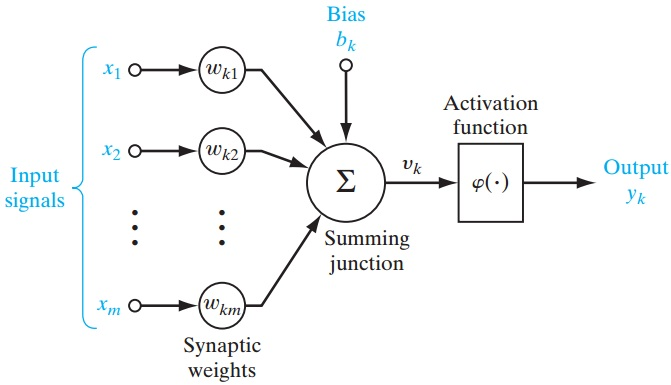
\includegraphics[scale=0.5]{../figures/neurone.jpg}
 \caption{Un neurone artificiel. \textbf{Source}: Haykin\cite{Haykin}}
 \label{neuronemlp}
\end{figure}
Un neurone effectue tout d'abord une somme pondérée de ses entrées \[v_k = b_k+\sum_{j=1}^{m}x_{j}w_{kj}\] où $x$ est le vecteur d'entrée de dimensions $m$.\\
Chaque terme $x_j$ est mutiplié par un poids $w_{kj}$.
Ce sont les poids qui seront modifiés lors de la phase d'apprentissage.
Le biais $b_k$ est souvent ajouté à la pondération.
Mais pour simplifier les formules, nous pouvons considèrer $b_k$ comme étant l'entrée $x_0 = 1$ de poid fixe $w_{k0} = 1$.
Et la somme pondérée est donc maintenant de la forme \[v_k = \sum_{j=0}^{m}x_{j}w_{kj}\]
Ensuite le neurone applique la \emph{fonction d'activation} $\phi$ sur la somme pondérée.
Le domaine de $y$ est généralement $[0,1]$ ou $[-1,1]$.\cite{Haykin,statistica}
La fonction $\phi$ utilisée dépend du problème qu'on veut résoudre (Figure \ref{mlpfonc}).
\begin{figure}
 \centering
 %insert tableau de statistica here
 \textbf{Fonctions d'activations.} (fonction de $x$)\\
 \begin{tabular}{|l|c|c|}
  Nom & Formule & Image\\
  \hline
  Identité & $x$ & $]-\infty,\infty[$\\
  \hline
  Sigmoïde & $\frac{1}{1+\exp^{-x}}$ & $]0,1]$\\
  \hline
  Tangente hyperbolique & $\frac{\exp^{x}-\exp^{-x}}{\exp^{x}+\exp^{-x}}$ & $]-1,1[$\\
  \hline
  Exponentielle & $e^{-x}$ & $]0,\infty[$\\
  \hline
  Sinus & $\sin{x}$ & $[-1,1]$\\
  \hline
  Softmax & $\frac{\exp^{x}}{\sum{\exp^{x_i}}}$ & $]0,1[$\\
  \hline
 \end{tabular}

 \caption{Fonctions d'activation principalement utilisés dans un MLP. \textbf{Source}: STATISTICA Réseaux de Neurones Automatisés (SANN)\cite{statistica}}
 \label{mlpfonc}
\end{figure}
\subsubsection{Structure}
\begin{figure}
 \centering
 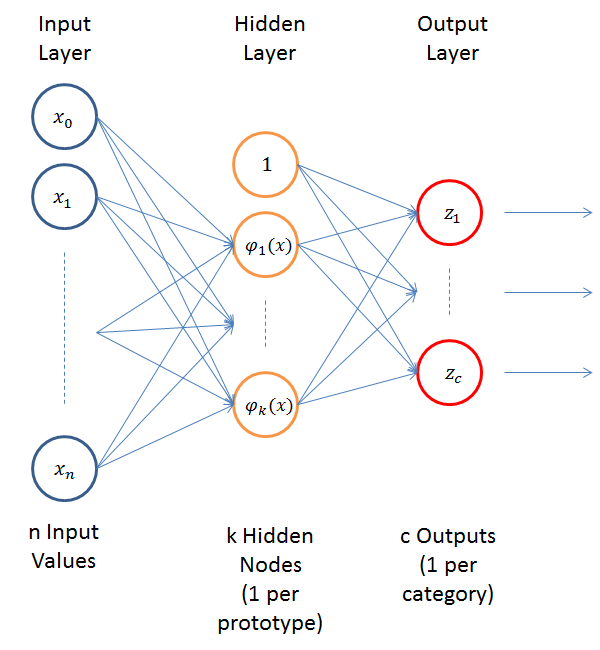
\includegraphics[scale=0.5]{../figures/nnstruct.png}
 \caption{Structure MLP à une couche cachée. \textbf{Source}: McCormick\cite{RBFtuto}}
 \label{structuremlp}
\end{figure}
Un \mlp est composé de plusieurs couches (Figure \ref{structuremlp}):
\begin{center}
 couche d'entrée $\rightarrow$ couches cachées $\rightarrow$ couche de sortie.
\end{center}
Un neurone envoie sa sortie vers tous les neurones de la couche suivante.
Il y a autant de neurones d'entrées que la dimension du vecteur d'entrée.
Le $k$\textsuperscript{ième} neurone d'entrée renvoie juste le $k$\textsuperscript{ième} élément du vecteur d'entrée.
Chaque neurone de sortie correspond à une dimension du vecteur de sortie.
Les neurones cachés et neurones de sortie correspondent à la Figure \ref{neuronemlp}.
\subsubsection{Apprentissage supervisé}\label{sec:appmlp}
Il existe plusieurs algorithmes pour changer les poids sur un réseau. Mais le plus connu est l'algorithme de de rétropropagation.\cite{Haykin,Gauthier}
Il s'agit d'un algorithme d'\emph{apprentissage supervisé}.
\begin{definition}
L'apprentissage supervisé est une méthode visant à améliorer un approximateur grâce à un calcul d'erreur (appelé aussi mesure de performance\cite{Gauthier}) comparant une sortie générée avec la sortie attendue.
\end{definition}
Nous avons donc besoin d'un ensemble de paires d'entrées/sorties.
L'algorithme applique la formule développée ci-dessous à tous les neurones sauf les neurones d'entrée.\\

Soit $\phi$, la fonction d'activation. Soit $\phi'$ la dérivée de $\phi$. Soit $Q$ l'\emph{erreur quadratique} utilisé comme mesure de performance.
\[Q = \frac{1}{2}\sum_{i}(\phi_i-s_i)^2\] où $\phi_i$ est la sortie du neurone de sortie $i$ et $s_i$ la sortie attendue pour la dimension $i$.
La modification du poid $W_{ij}$ vaut \[\Delta W_{ij} = -\eta\partiel{Q}{W_{ij}}\] où $\eta$ est une constante appelé \emph{pas du gradient}.
Par le théorème de dérivation des fonctions composées, \[\partiel{Q}{W_{ij}} = \partiel{Q}{\phi_i} \partiel{\phi_i}{v_i} \partiel{v_i}{W_{ij}}\]
\begin{thm}[dérivation des fonctions composées]
Soit $f:A~\rightarrow~B : y~\rightarrow~f(y)$ et $g:B~\rightarrow~C : x~\rightarrow~g(x)$. Alors la dérivée de $f~\circ~g$ en $x$ vaut
\[\partiel{f}{x} = \partiel{f}{g} \partiel{g}{x}\]
\end{thm}
Posons $\delta_i = \partiel{Q}{\phi_i} \partiel{\phi_i}{v_i}$. $\delta_i$ est appelé \emph{contridution à l'erreur} du neurone $i$ et est utilisé pour l'apprentissage des neurones de la couche prédédente.
Ensuite, soit $x_i$ l'entrée du neurone $i$,
\begin{equation}
 \begin{split}
  \partiel{v_i}{W_{ij}} & = \partiel{(W_{i0}x_i)}{W_{ij}} + \partiel{(W_{i1}x_i)}{W_{ij}} + ... + \partiel{(W_{ij}x_i)}{W_{ij}} + ... + \partiel{(W_{im}x_m)}{W_{ij}}\\
  ~ & = x_i
  \end{split}
\end{equation}
On a donc \[\Delta W_{ij} = -\eta \delta_i x_i\].
Déterminons la valeur de $\delta_i$.\\

\textbf{Si le neurone $i$ est un neurone de sortie,}
Soit $m$ la dimension de l'entrée $x$ (du neurone). Soit $l$ la dimension du vecteur de sortie du réseau.
\begin{equation}
 \begin{split}
  \partiel{Q}{\phi_i} & = \frac{1}{2} \left( \partiel{(\phi_0 - s_0)^2}{\phi_i} + \partiel{(\phi_1 - s_1)^2}{\phi_i} + ... + \partiel{(\phi_i - s_i)^2}{\phi_i} + ... + \partiel{(\phi_l - s_l)^2}{\phi_i} \right)\\
  ~ & = \frac{1}{2}2(\phi_i - s_i)\partiel{(\phi_i - s_i)}{\phi_i}\\
  ~ & = (\phi_i - s_i) 1\\
  \partiel{\phi_i}{v_i} & = \phi'(v_i)
 \end{split}
\end{equation}\label{eq:a}
On obtient donc \[\delta_i = (\phi_i - s_i)\phi'(v_i)\]\\

\textbf{Si le neurone $i$ est un neurone caché,}
Soit $m$ la dimension de l'entrée $x$ (du neurone). Soit $n$ le nombre de neurone de la couche suivante.
L'indice $k$ sera utilisé pour désigner un neurone de la couche suivante.
\begin{equation}
 \begin{split}
  \partiel{Q}{\phi_i} & = \sum_{k=1}^{n} \partiel{Q}{\phi_k} \partiel{\phi_k}{v_k} \partiel{v_k}{\phi_i}\\
  ~ & = \sum_{k=1}^{n} \delta_k \partiel{v_k}{\phi_i}
 \end{split}
\end{equation}
Or $\phi_i$ est l'entrée du neurone $k$ recevant la sortie du neurone $i$. Posons $W_{ki}$ le poid que $k$ attribue à $\phi_i$.
On obtient donc \[\partiel{v_k}{\phi_i} = \partiel{W_{ki}\phi_i}{\phi_i} = W_{ki}\]
Comme pour les neurones de sorties, $\partiel{\phi_i}{v_i} = \phi_i'(v_i)$.
Et du coup, \[\delta_i = \phi_i'(v_i) \sum_{k=1}^{n} \delta_k W_{ki}\]
\subsubsection{Apprentissage non supervisé}
Il existe également des algorithmes d'apprentissage non supervisé.
Ces algorithmes ne cherche pas à minimiser une erreur mais maximisent un score calculé à partir de la sortie du réseau.
\subsubsection{Apprentissage sur plusieurs MLP}
Lorque l'une des dimensions du vecteur d'entrée est discrète et finie, il est conseillé d'utiliser un \mlp différent par valeur différente sur cette dimension.\cite{Gauthier}
Cette technique peut aussi être utilisé si nous pouvons classer tous les états possibles selon le contexte.
Par exemple, pour la Sphero nous pourrions utiliser un \mlp pour le contexte \enum{en train de déraper} et un autre \mlp pour le contexte \enum{ne dérape pas}.
\subsubsection{Applications}
À une couche cachée, un \mlp peut déja servir pour la classification non linéaire.\cite{statistica}\\
Les \mlp sont aussi utilisés en commande de robot par caméra.\cite{Pomerleau}
\subsection{Fonctions à base radiale}
Nous désignerons un réseau de neurones \emph{fonctions à base radiale} par sa terminologie anglaise: \rbf pour \enum{Rasial Basis Function}.
\newcommand{\factnorm}{\sum_{r=1}^{m}x_{r}}
\subsubsection{Neurone}
Un neurone \textbf{caché} d'un \rbf n'effectue pas de somme pondérée de ses entrées.
Il applique directement sa fonction d'activation $\phi$, une gaussienne de moyenne $\mu$ et d'écart-type $\sigma$ où $x$, de dimension $n$, est l'entrée du neurone.
\begin{equation}\label{eq:cachephi}
 \phi(x) = e^{-\frac{1}{2}\sum_{k=1}^{n}\frac{(x_k-\mu_{ik})^2}{\sigma_{ik}^{2}}}
\end{equation}
Où $i$ est l'indice du neurone. $\mu$ s'appelle aussi \emph{prototype} dans le cas d'un \rbf.
%$\phi(x)$ peut se résumer en: \[\phi(x) = e^{-\beta||x-\mu||^2}\]Où $\beta$ est donc un coefficient qui règle la largeur de la courbe en cloche.\\
\\

Un neurone \textbf{de sortie} d'un \rbf n'effectue pas non plus de somme pondérée de ses entrées. Sa fonction d'activation est:
À une couche cachée, un \mlp peut déja servir pour la classification non linéaire.\cite{statistica}\\
\begin{equation}\label{eq:sortiephi}
 \phi(x) = \frac{\sum_{j=1}^{m}W_{ij}x_{j}}{\sum_{j=1}^{m}x_{j}}
\end{equation}
Où $i$ est l'indice du neurone et $x$ l'entrée de dimension $m$.
\begin{figure}
 \centering
 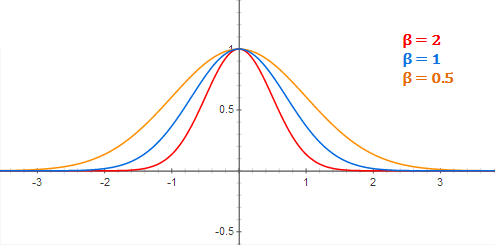
\includegraphics[scale=0.7]{../figures/RBFactivation.png}%TODO generer ça soit-même
 \caption{Activation d'un neurone RBF avec différentes valeurs d'écart-type}
 \label{rbfactivation}
\end{figure}
La Figure \ref{rbfactivation} représente la sortie d'un neurone \rbf où $\mu$ et $x$ sont de dimension 1 et $\mu = 0$.\\
Pour résumer, un neurone \rbf renvoie une valeur indiquant la simularité entre l'entrée et son prototype.
\subsubsection{Structure}
\begin{figure}
 \centering
 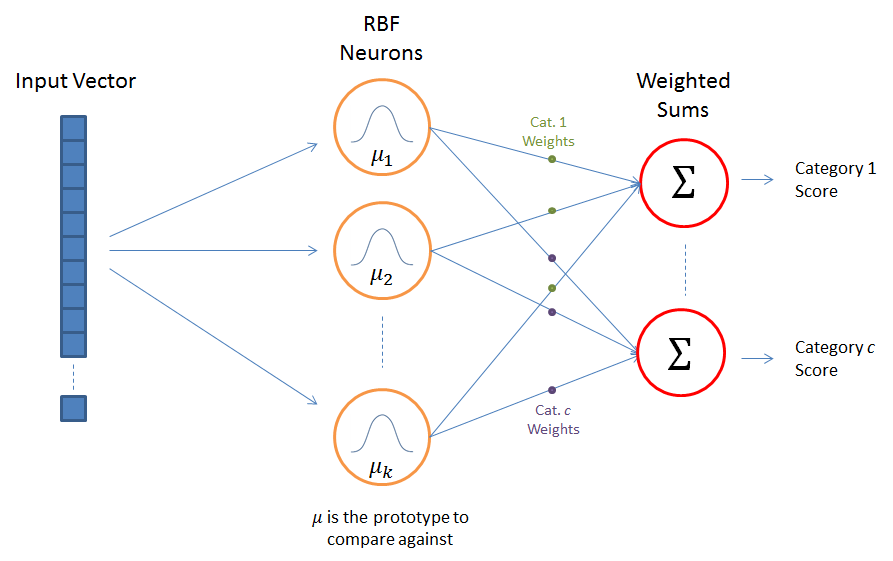
\includegraphics[scale=0.5]{../figures/RBFstruct.png}
 \caption{Structure RBF. \textbf{Source}: McCormick\cite{RBFtuto}}
 \label{structurerbf}
\end{figure}
La structure d'un \rbf est comme celle du \mlp sauf qu'il n'y a qu'une seule couche cachée (Figure \ref{structurerbf}).
\subsubsection{Apprentissage}
Dans ce réseau, les paramètres qui seront modifiés lors de l'apprentissage sont les poids des neurones de sortie et les moyennes et écart-types des neurones cachés.
L'algorithme de rétropropagation peut être utilisé pour un apprentissage supervisé d'un \rbf.
Reprenons \eqref{eq:Q}, l'erreur quadratique $Q$ défini dans la section \ref{sec:appmlp}.
En reprenant le même raisonnement que la rétropropagation dans un \mlp,
on va faire un pas de $\eta$ dans le sens opposé et proportionnel au gradient pour chaque poid $W_{ij}$ des neurones de sortie mais aussi des prototypes $\mu_i$ et écart-types $\sigma_i$ des neurones cachés.
C'est à dire que les paramètres seront modifiés de la sorte:
\begin{equation}%\label{eq:modifpoid}
 \Delta W_{ij} = -\eta \partiel{Q}{W_{ij}}
\end{equation}
\begin{equation}%\label{eq:modifmu}
 \Delta \mu_{ik} = -\eta \partiel{Q}{\mu_{ik}}
\end{equation}
\begin{equation}%\label{eq:modifsigma}
 \Delta \sigma_{ik} = \eta \partiel{Q}{\sigma_{ik}}
\end{equation}

Le dévellopement des formules de rétropropagation a été fait en annexe \ref{sec:eqrbf}.
Et voici ce que nous obtenons au final:\\
Pour un neurone de sortie :
\[\Delta W_{ij} = -\eta (\phi_i - s_i) \frac{x_j}{\factnorm}\]
Pour un neurone caché, posons $x_r$ l'entrée de $j$ provenant de $i$ (c'est à dire $\phi_i = x_r$),\\
posons $n$ la dimension de l'entrée de $j$,\\
posons aussi $R = \sum_{k=1}^{n}x_k$.
\[\Delta\mu_{ik} = -\eta \left[\sum_{i}(\phi_j - s_j) \frac{1}{R^2} \left(W_{jr}R - \sum_{k=1}^{n}W_{jk}x_k\right)\right] \phi_i\frac{x_k-\mu_{ik}}{\sigma_{ik}^2}\]
\[\Delta \sigma_{ik} = -\eta \left[\sum_{i}(\phi_j - s_j) \frac{1}{R^2} \left(W_{jr}R - \sum_{k=1}^{n}W_{jk}x_k\right)\right] \phi_i \frac{(x_k-\mu_{ik})^2}{\sigma_{ik}^3}\]

\subsubsection{Applications}
Un \rbf peut aussi servir pour la commande de robot.\cite{Gauthier}

Un des inconvénients des \rbf est que le nombre de neurones cachés croît avec la dimension et la taille du vecteur d'entrée puisqu'un neurone caché s'active seulement pour des entrées dans le voisinage de son prototype.
Nous pouvons raisonablement envisager ce modèle pour notre application puisque la description de l'état actuel et de l'état cible contiendra typiquement une coordonnée, un vecteur vitesse, une orientation et éventuellement l'accéleration, etc...
La taille de l'entrée sera donc relativement petite. Ce sera lors de la phase pratique qu'on évaluera le nombre de neurones cachés nécessaires.
De plus, les \rbf sont moins sensibles au bruit.\cite{adversarial}
\subsection{Convolutif (CNN)}
\subsubsection{Réseau de neurones récurrent (RNN)}
Jusque maintenant, nous avons vu des réseaux de neurones \emph{feedforward}.
C'est à dire qu'ils ne présentent aucune boucle. Mais il éxiste des réseaux de neurones présentant des boucles.
Cela leur permet de prendre en compte les entrées précédentes.
\ssstitle{Structure}
\begin{figure}
 \centering
 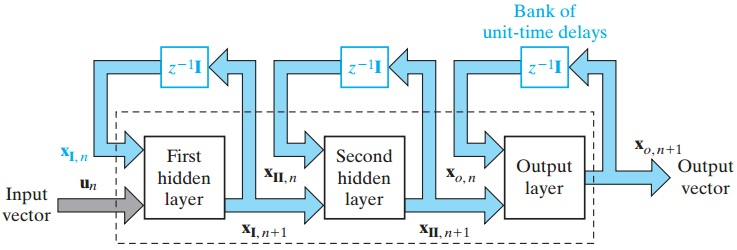
\includegraphics[scale=0.5]{../figures/structurermlp.jpg}
 \caption{Structure RLMP. \textbf{Source}: Haykin. p795\cite{Haykin}}
 \label{structurermlp}
\end{figure}
\begin{figure}
 \centering
 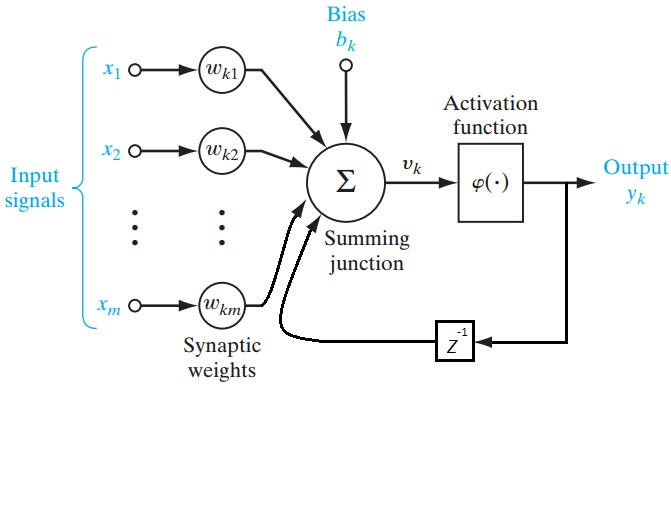
\includegraphics[scale=0.5]{../figures/neuronermlp.jpg}
 \caption{Neurone caché d'un RMLP}
 \label{neuronermlp}
\end{figure}
Un réseau de neurones récurrent est un réseaux présentant des boucles dans sa structure.
Des \emph{délais} notés $Z^{-1}$ sont présents sur certains arcs dans le réseau afin de retarder d'une étape, la transmission d'une valeur.
Une étape dans un réseau consiste à recevoir une entrée et de générer une sortie.
Il existe plusieurs réseaux de type récurrent (récurrent simple, machine à états liquide, etc).
La Figure \ref{structurermlp} présente un réseau de type perceptron multi-couches récurrent (\rmlp).
Il s'agit d'un \mlp dont les neurones des couches cachées ont un arc qui boucle sur le neurone lui-même avec un $Z^{-1}$ sur cet arc, comme sur la Figure \ref{neuronermlp}.
\ssstitle{Applications}
Grâce aux délais, le réseau peut approximer des fonctions dont la sortie ne dépend pas seulement de l'entrée actuelle mais aussi des entrées précédentes.
Mais cette fonctionnalité n'est pas utile pour notre application puisque les commandes à générer ne dépendent pas des états précédents l'état actuel.
%Les \emph{machines à états liquides} (\lsm), dont les connections se font de manière aléàtoire, sont utilisés pour la reconnaissance automatique de la parole. %TODO citer
%Les \emph{long-short term memory} sont utilisés pour la reconnaissance automatique de la parole ou de l'écriture manuscrite. %TODO citer
\subsection{CMAC}
\section{Architectures}

\section{Choix du réseau}
Nous n'avons pas besoin d'un réseau de neurones récurrent. Les commandes à appliquer au moment $t$ ne dépendent pas de la vitesse, position et autres données fournies à $t-T$.
Le réseau le mieux adapté pour notre problème est un réseau de neurones à base radial.
En effet, les \rbf sont moins sensibles au bruit que les \mlp \cite{adversarial,Gauthier}.%gauthier p 39,40
%TODO pourquoi
Un inconvénient des \rbf, celui du nombre de neurones cachés qui croît avec la dimension et la taille du vecteur d'entrée, ne pose pas de problème dans notre cas
car le nombre de dimensions est faible
et le domaine d'entrée est assez faible pour chaque dimensions.
\section{Choix de l'API}
Les APIs officiels sont:\cite{SDKofficiels} \textbf{Objective-C}, \textbf{Swift}, \textbf{Android}.\\
Il existe également des APIs créé par la communauté:\cite{gosphero} \textbf{C\#}, \textbf{JavaScript}, \textbf{Ruby}, \textbf{Python}\cite{pythonAPI}, \textbf{Arduino}, \textbf{C++}\cite{cppAPI}.\\
%TODO
\section{Avancement du projet et perspective}
\subsection*{Remerciements}
\noindent Je remercie monsieur Pierre \textsc{Hauweele} de m'avoir proposé un projet qui est exactement dans le domaine que je voulais, de son aide et d'avoir choisi d'être directeur de mon projet.\\

\noindent Je remercie monsieur Hadrien Mélot d'être directeur de mon projet et de l'aide qu'il m'a apporté.\\

\noindent Je remercie monsieur Tom Mens d'être rapporteur de mon projet et de son aide.\\

\bibliographystyle{plain}
\bibliography{../bibli}
\end{document}
